\begin{frame}{Causal Masking}
  \begin{itemize}
    \item<1> \textbf{Purpose:} Prevents the model from attending to future tokens in the sequence.
    \item<2> \textbf{Implementation:} Uses a triangular mask in the self-attention mechanism.
    \item<3> \textbf{Effect:} Ensures that predictions for a token only depend on previous tokens, maintaining the autoregressive property.
  \end{itemize}
\end{frame}

\begin{frame}{Causal Masking}
  \centering
  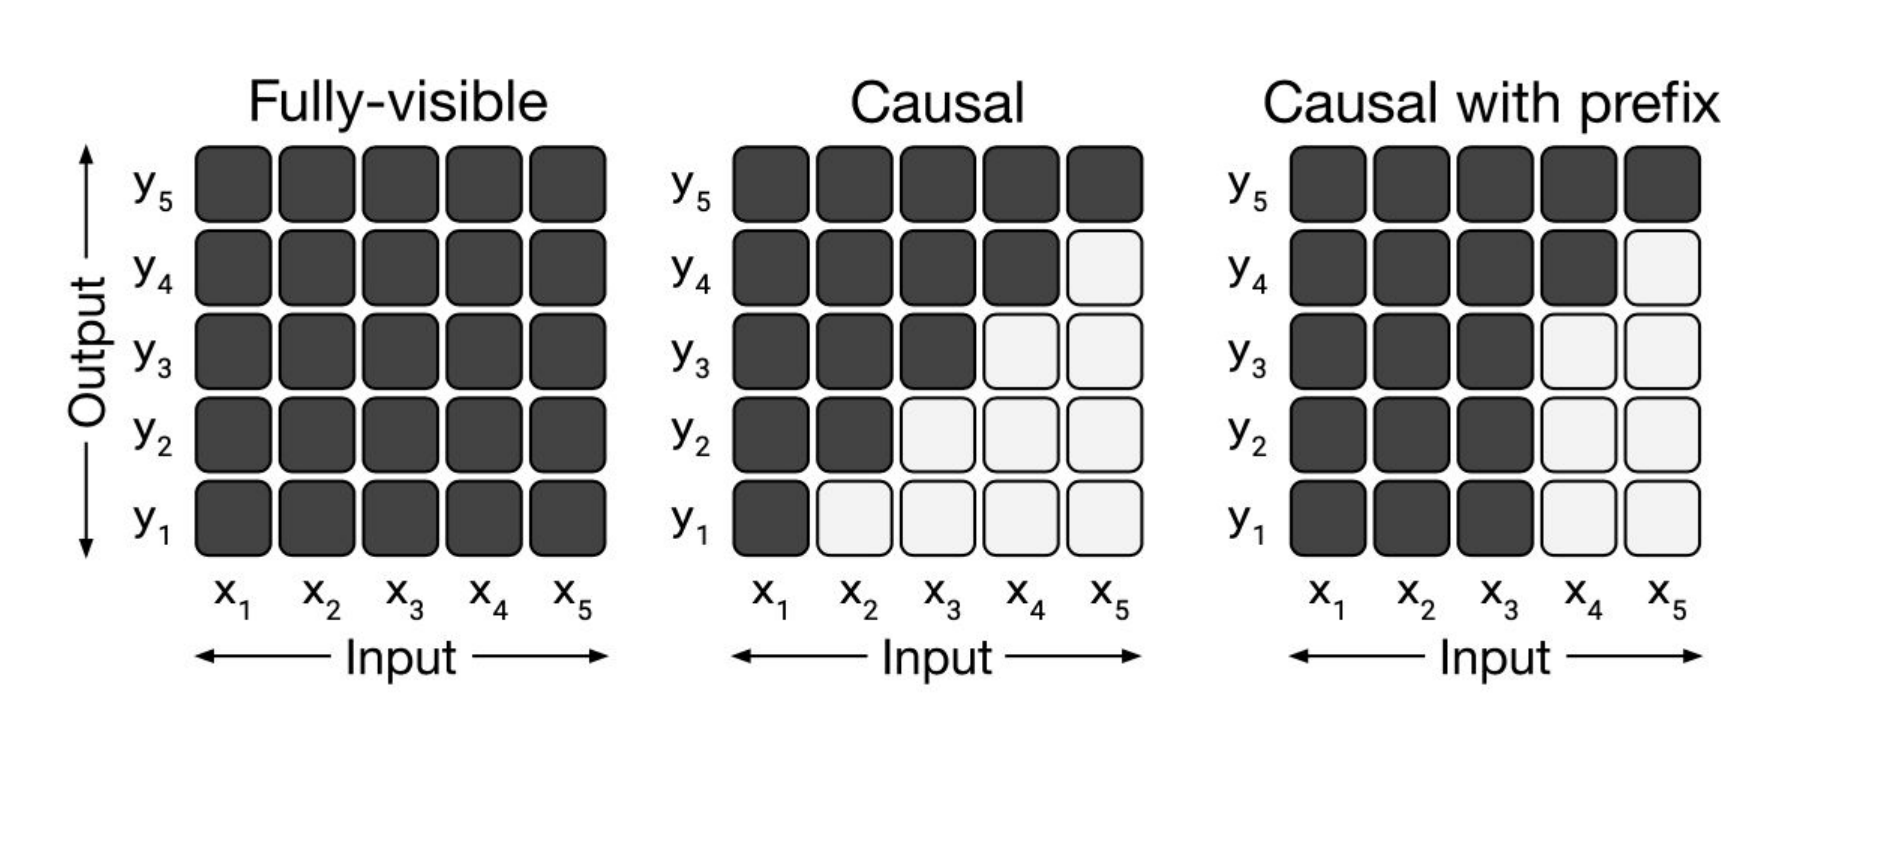
\includegraphics[width=\paperwidth,height=0.95\paperheight,keepaspectratio]{images/introduction-to-transformers/transformer_attention_masks_fully_visible_causal_prefix.png}
\end{frame}

\begin{frame}{Causal Masking}
  \centering
  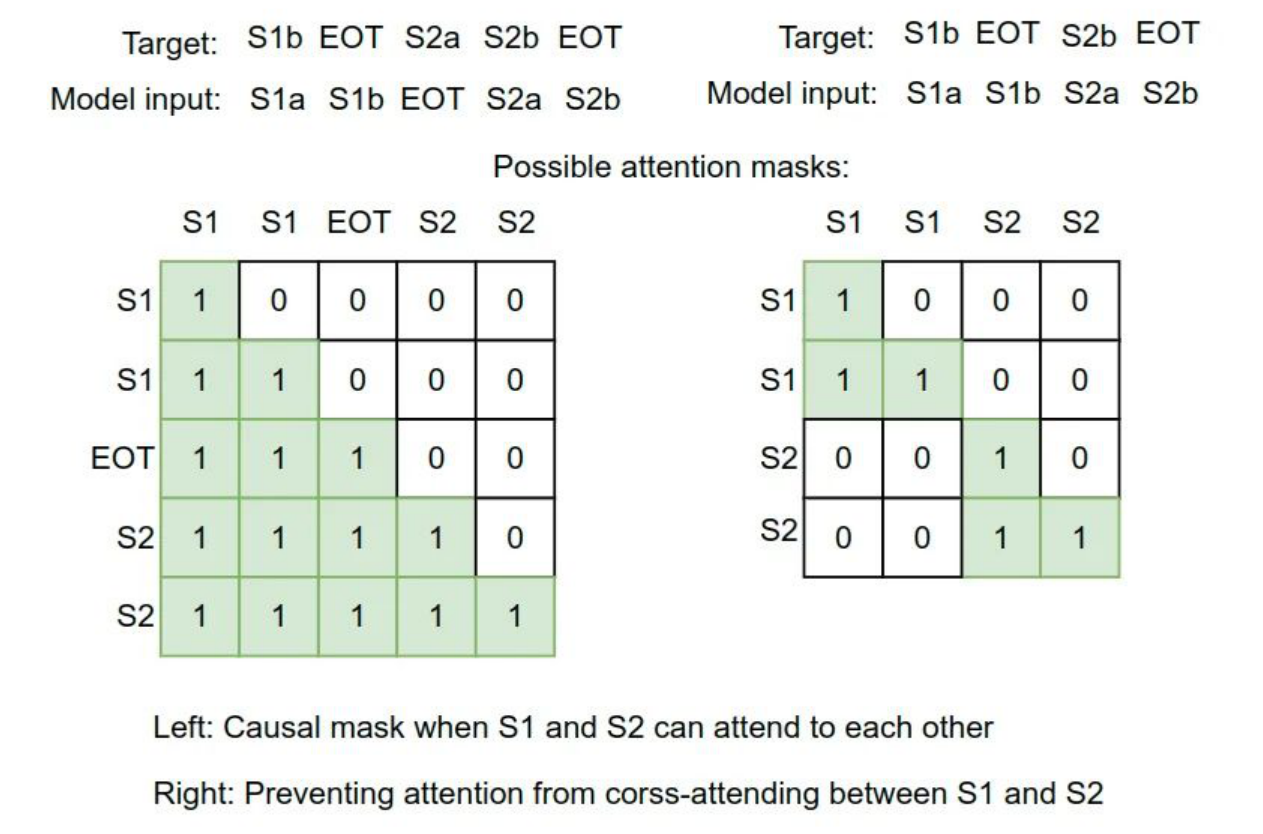
\includegraphics[width=0.8\paperwidth,height=0.8\paperheight,keepaspectratio]{images/introduction-to-transformers/transformer_attention_mask_matrices_causal_vs_cross_segment.png}
\end{frame}

